% CNETA pipeline figure: how the programs and scripts chain together, and
% which files cross the boundaries between them.
%
% Draft for the researcher meeting; the docs do not use it yet. Plain
% pdflatex on TeX Live "basic" (TikZ + Latin Modern, nothing else). Do not
% run this file directly; ./build.sh renders both schemes. To render one:
%
%   pdflatex -jobname=cneta-pipeline-dark \
%     "\def\PipelineScheme{dark}% CNETA pipeline figure: how the programs and scripts chain together, and
% which files cross the boundaries between them.
%
% Draft for the researcher meeting; the docs do not use it yet. Plain
% pdflatex on TeX Live "basic" (TikZ + Latin Modern, nothing else). Do not
% run this file directly; ./build.sh renders both schemes. To render one:
%
%   pdflatex -jobname=cneta-pipeline-dark \
%     "\def\PipelineScheme{dark}% CNETA pipeline figure: how the programs and scripts chain together, and
% which files cross the boundaries between them.
%
% Draft for the researcher meeting; the docs do not use it yet. Plain
% pdflatex on TeX Live "basic" (TikZ + Latin Modern, nothing else). Do not
% run this file directly; ./build.sh renders both schemes. To render one:
%
%   pdflatex -jobname=cneta-pipeline-dark \
%     "\def\PipelineScheme{dark}% CNETA pipeline figure: how the programs and scripts chain together, and
% which files cross the boundaries between them.
%
% Draft for the researcher meeting; the docs do not use it yet. Plain
% pdflatex on TeX Live "basic" (TikZ + Latin Modern, nothing else). Do not
% run this file directly; ./build.sh renders both schemes. To render one:
%
%   pdflatex -jobname=cneta-pipeline-dark \
%     "\def\PipelineScheme{dark}\input{cneta-pipeline}"
%
%   \PipelineScheme  light | dark   (default light): colours for a light or a
%                    dark background; the background itself stays transparent.
%
% Box colours follow the house convention of the report kit:
%   blue   a program step        grey    a file (the contract between steps)
%   purple a script in util/     green   a result people look at
%   amber  settings to choose    red, dashed   not released yet

\providecommand\PipelineScheme{light}

\documentclass[tikz,border=5mm]{standalone}
\usepackage[T1]{fontenc}
\usepackage{lmodern}
\renewcommand*\familydefault{\sfdefault}
\usetikzlibrary{arrows.meta,positioning,calc,shapes.misc}
\hyphenpenalty=10000
\exhyphenpenalty=10000

% ---------------------------------------------------------------- palette
\def\schemeLight{light}
\ifx\PipelineScheme\schemeLight
  \definecolor{ink}{HTML}{16222E}  \definecolor{muted}{HTML}{6B7280}
  \definecolor{stln}{HTML}{24405C} \definecolor{stfl}{HTML}{E7EEF5}  % program
  \definecolor{syln}{HTML}{55606D} \definecolor{syfl}{HTML}{EDEFF2}  % file
  \definecolor{deln}{HTML}{A5690C} \definecolor{defl}{HTML}{FDF3E2}  % settings
  \definecolor{galn}{HTML}{A83226} \definecolor{gafl}{HTML}{FAE9E7}  % draft
  \definecolor{opln}{HTML}{2C6B4F} \definecolor{opfl}{HTML}{E6F1EB}  % result
  \definecolor{ppln}{HTML}{5B4B8A} \definecolor{ppfl}{HTML}{EEEAF6}  % script
\else
  \definecolor{ink}{HTML}{E6EBF0}  \definecolor{muted}{HTML}{A9B4BF}
  \definecolor{stln}{HTML}{8FB3D9} \definecolor{stfl}{HTML}{25364A}
  \definecolor{syln}{HTML}{A0AAB5} \definecolor{syfl}{HTML}{333B45}
  \definecolor{deln}{HTML}{E0A94B} \definecolor{defl}{HTML}{40321A}
  \definecolor{galn}{HTML}{E07A6E} \definecolor{gafl}{HTML}{42241F}
  \definecolor{opln}{HTML}{6FBF93} \definecolor{opfl}{HTML}{1F3A2B}
  \definecolor{ppln}{HTML}{B3A3E0} \definecolor{ppfl}{HTML}{302A45}
\fi

% ---------------------------------------------------------------- styles
\tikzset{
  x=1mm, y=1mm,
  every node/.style={text=ink, font=\small, align=center, inner sep=4pt,
                     rounded corners=2pt, line width=0.8pt},
  prog/.style={draw=stln, fill=stfl, line width=1pt},
  file/.style={draw=syln, fill=syfl, font=\footnotesize},
  script/.style={draw=ppln, fill=ppfl},
  result/.style={draw=opln, fill=opfl},
  settings/.style={draw=deln, fill=defl, font=\footnotesize},
  draft/.style={draw=galn, fill=gafl, dash pattern=on 3pt off 2pt},
  dcap/.style={text=muted, font=\scriptsize, inner sep=1pt},
  lane/.style={text=muted, font=\footnotesize\bfseries, inner sep=1pt, anchor=west},
  arr/.style={-{Stealth[length=2.2mm,width=1.7mm]}, line width=0.8pt, draw=stln},
  arrf/.style={-{Stealth[length=2.2mm,width=1.7mm]}, line width=0.7pt, draw=syln},
  arro/.style={-{Stealth[length=2.2mm,width=1.7mm]}, line width=0.8pt, draw=opln},
  arrd/.style={-{Stealth[length=2.2mm,width=1.7mm]}, line width=0.8pt, draw=galn,
               dash pattern=on 3pt off 2pt},
  tt/.style={font=\footnotesize\ttfamily},
  % legend swatch: a small box in one of the styles above
  chip/.style={minimum width=7mm, minimum height=3.6mm, inner sep=0pt,
               rounded corners=1pt},
  lg/.style={anchor=west, text=ink, font=\footnotesize, inner sep=1pt},
}
\newcommand{\f}[1]{{\ttfamily #1}}

\begin{document}
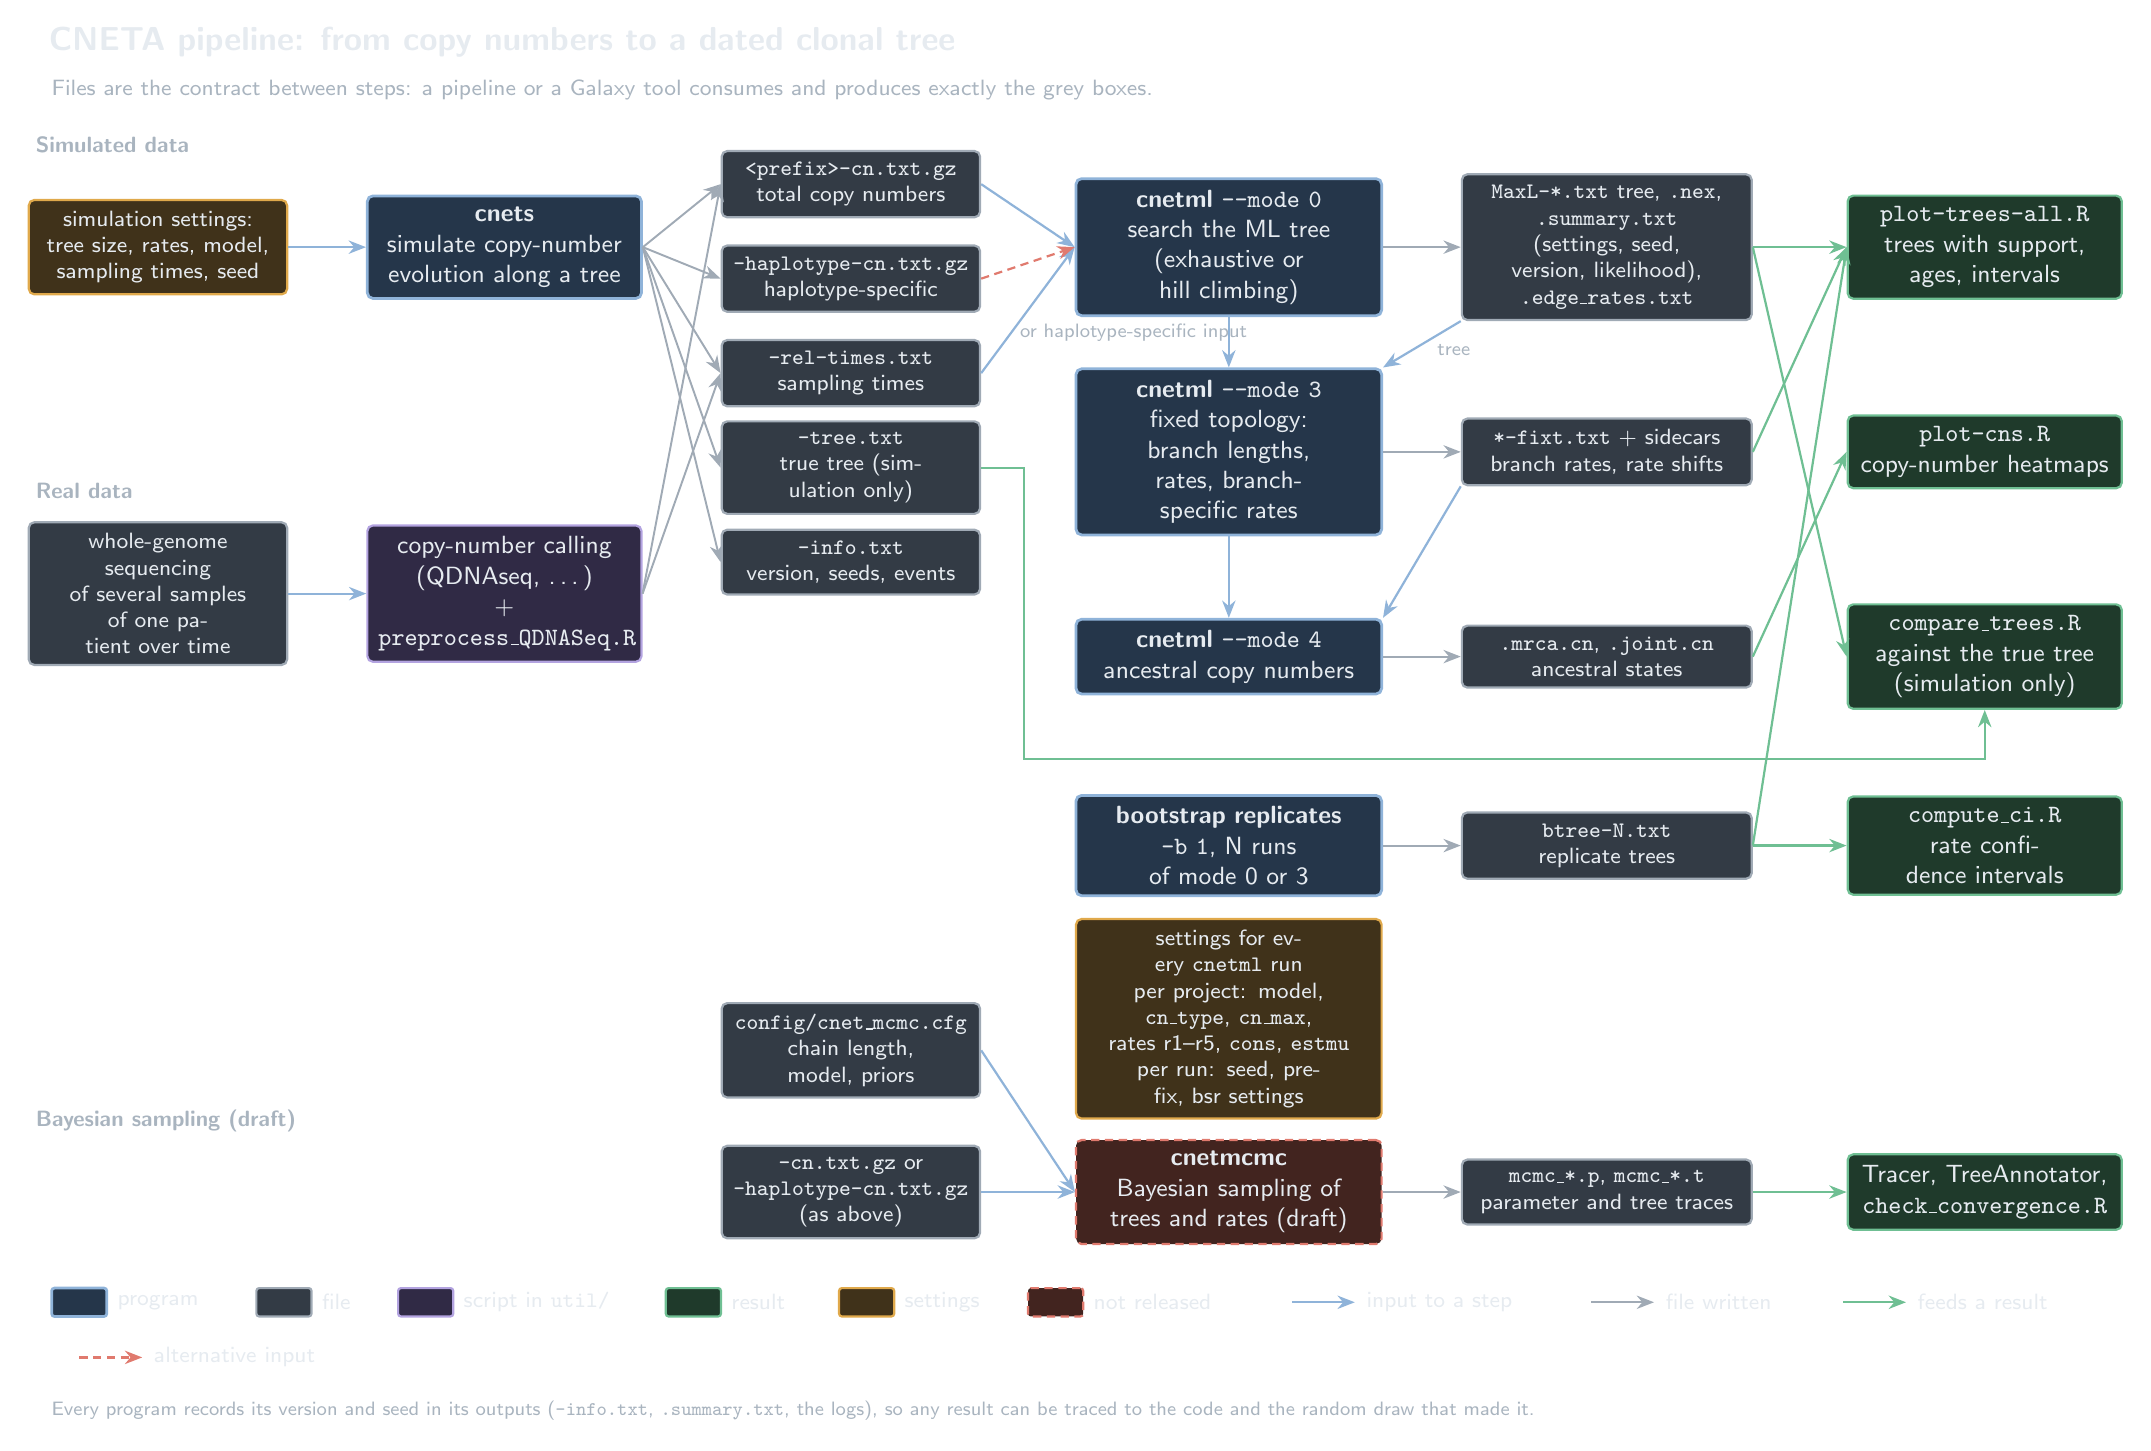
\begin{tikzpicture}

% ---------------------------------------------------------------- title
\node[anchor=west, font=\large\bfseries, inner sep=0pt] at (0,26)
  {CNETA pipeline: from copy numbers to a dated clonal tree};
\node[anchor=west, dcap, font=\footnotesize] at (0,20)
  {Files are the contract between steps: a pipeline or a Galaxy tool consumes and produces exactly the grey boxes.};

% ---------------------------------------------------------------- lanes
\node[lane] at (-2,13) {Simulated data};
\node[lane] at (-2,-31) {Real data};
\node[lane] at (-2,-111) {Bayesian sampling (draft)};

% ---------------------------------------------------------------- column A: sources
\node[settings, text width=30mm] (simset) at (14,0)
  {simulation settings:\\tree size, rates, model,\\sampling times, seed};
\node[file, text width=30mm] (wgs) at (14,-44)
  {whole-genome sequencing\\of several samples\\of one patient over time};

% ---------------------------------------------------------------- column B: producers
\node[prog, text width=32mm] (cnets) at (58,0)
  {\textbf{cnets}\\simulate copy-number\\evolution along a tree};
\node[script, text width=32mm] (prep) at (58,-44)
  {copy-number calling\\(QDNAseq, \ldots)\\+ \f{preprocess\_QDNASeq.R}};

% ---------------------------------------------------------------- column C: input files
\node[file, text width=30mm] (fcn) at (102,8)
  {\f{<prefix>-cn.txt.gz}\\total copy numbers};
\node[file, text width=30mm] (fhap) at (102,-4)
  {\f{-haplotype-cn.txt.gz}\\haplotype-specific};
\node[file, text width=30mm] (ftimes) at (102,-16)
  {\f{-rel-times.txt}\\sampling times};
\node[file, text width=30mm] (ftree) at (102,-28)
  {\f{-tree.txt}\\true tree (simulation only)};
\node[file, text width=30mm] (finfo) at (102,-40)
  {\f{-info.txt}\\version, seeds, events};

% ---------------------------------------------------------------- column D: cnetml
\node[prog, text width=36mm] (m0) at (150,0)
  {\textbf{cnetml} \f{--mode 0}\\search the ML tree\\(exhaustive or hill climbing)};
\node[prog, text width=36mm] (m3) at (150,-26)
  {\textbf{cnetml} \f{--mode 3}\\fixed topology: branch lengths,\\rates, branch-specific rates};
\node[prog, text width=36mm] (m4) at (150,-52)
  {\textbf{cnetml} \f{--mode 4}\\ancestral copy numbers};
\node[prog, text width=36mm] (boot) at (150,-76)
  {\textbf{bootstrap replicates}\\\f{-b 1}, N runs of mode 0 or 3};
\node[settings, text width=36mm] (params) at (150,-98)
  {settings for every \f{cnetml} run\\per project: model, \f{cn\_type}, \f{cn\_max},\\rates r1--r5, \f{cons}, \f{estmu}\\per run: seed, prefix, bsr settings};

% ---------------------------------------------------------------- column E: outputs
\node[file, text width=34mm] (o0) at (198,0)
  {\f{MaxL-*.txt} tree, \f{.nex},\\\f{.summary.txt} (settings, seed,\\version, likelihood), \f{.edge\_rates.txt}};
\node[file, text width=34mm] (o3) at (198,-26)
  {\f{*-fixt.txt} + sidecars\\branch rates, rate shifts};
\node[file, text width=34mm] (o4) at (198,-52)
  {\f{.mrca.cn}, \f{.joint.cn}\\ancestral states};
\node[file, text width=34mm] (ob) at (198,-76)
  {\f{btree-N.txt}\\replicate trees};

% ---------------------------------------------------------------- column F: analysis
\node[result, text width=32mm] (plott) at (246,0)
  {\f{plot-trees-all.R}\\trees with support,\\ages, intervals};
\node[result, text width=32mm] (plotc) at (246,-26)
  {\f{plot-cns.R}\\copy-number heatmaps};
\node[result, text width=32mm] (cmp) at (246,-52)
  {\f{compare\_trees.R}\\against the true tree\\(simulation only)};
\node[result, text width=32mm] (ci) at (246,-76)
  {\f{compute\_ci.R}\\rate confidence intervals};

% ---------------------------------------------------------------- MCMC lane
\node[file, text width=30mm] (cfg) at (102,-102)
  {\f{config/cnet\_mcmc.cfg}\\chain length, model, priors};
\node[file, text width=30mm] (cnin) at (102,-120)
  {\f{-cn.txt.gz} or\\\f{-haplotype-cn.txt.gz}\\(as above)};
\node[draft, text width=36mm] (mcmc) at (150,-120)
  {\textbf{cnetmcmc}\\Bayesian sampling of\\trees and rates (draft)};
\node[file, text width=34mm] (traces) at (198,-120)
  {\f{mcmc\_*.p}, \f{mcmc\_*.t}\\parameter and tree traces};
\node[result, text width=32mm] (tracer) at (246,-120)
  {Tracer, TreeAnnotator,\\\f{check\_convergence.R}};

% ---------------------------------------------------------------- arrows
\draw[arr] (simset) -- (cnets);
\foreach \t in {fcn,fhap,ftimes,ftree,finfo} {\draw[arrf] (cnets.east) -- (\t.west);}
\draw[arr] (wgs) -- (prep);
\draw[arrf] (prep.east) -- (fcn.west);
\draw[arrf] (prep.east) -- (ftimes.west);

\draw[arr] (fcn.east) -- (m0.west);
\draw[arr] (ftimes.east) -- (m0.west);
\draw[arrd] (fhap.east) -- (m0.west);
\node[dcap,anchor=south west] at (123,-12.5) {or haplotype-specific input};

\draw[arrf] (m0) -- (o0);
\draw[arr] (o0.south west) -- (m3.north east);
\node[dcap,anchor=west] at (176,-13) {tree};
\draw[arrf] (m3) -- (o3);
\draw[arr] (o3.south west) -- (m4.north east);
\draw[arrf] (m4) -- (o4);
\draw[arrf] (boot) -- (ob);
\draw[arr] (m0) -- (m3);
\draw[arr] (m3) -- (m4);

\draw[arro] (o0.east) -- (plott.west);
\draw[arro] (o3.east) -- (plott.west);
\draw[arro] (ob.east) -- (plott.west);
\draw[arro] (ob.east) -- (ci.west);
\draw[arro] (o4.east) -- (plotc.west);
\draw[arro] (o0.east) -- (cmp.west);
\draw[arro] (ftree.east) -- (124,-28) -- (124,-65) -- (246,-65) -- (cmp.south);

\draw[arr] (cfg.east) -- (mcmc.west);
\draw[arr] (cnin.east) -- (mcmc.west);
\draw[arrf] (mcmc) -- (traces);
\draw[arro] (traces) -- (tracer);

% ---------------------------------------------------------------- legend
\begin{scope}[shift={(0,-134)}]
  \node[prog, chip]     (lg1) at (4,0)   {}; \node[lg] at ([xshift=2pt]lg1.east) {program};
  \node[file, chip]     (lg2) at (30,0)  {}; \node[lg] at ([xshift=2pt]lg2.east) {file};
  \node[script, chip]   (lg3) at (48,0)  {}; \node[lg] at ([xshift=2pt]lg3.east) {script in \f{util/}};
  \node[result, chip]   (lg4) at (82,0)  {}; \node[lg] at ([xshift=2pt]lg4.east) {result};
  \node[settings, chip] (lg5) at (104,0) {}; \node[lg] at ([xshift=2pt]lg5.east) {settings};
  \node[draft, chip]    (lg6) at (128,0) {}; \node[lg] at ([xshift=2pt]lg6.east) {not released};
  \draw[arr]  (158,0) -- ++(8,0); \node[lg] at (167,0) {input to a step};
  \draw[arrf] (196,0) -- ++(8,0); \node[lg] at (205,0) {file written};
  \draw[arro] (228,0) -- ++(8,0); \node[lg] at (237,0) {feeds a result};
  \draw[arrd] (4,-7) -- ++(8,0);  \node[lg] at (13,-7) {alternative input};
\end{scope}

% ---------------------------------------------------------------- footer
\node[dcap,anchor=north west, align=left] at (0,-146)
  {Every program records its version and seed in its outputs (\f{-info.txt}, \f{.summary.txt}, the logs), so any result can be traced to the code and the random draw that made it.};

\end{tikzpicture}
\end{document}
"
%
%   \PipelineScheme  light | dark   (default light): colours for a light or a
%                    dark background; the background itself stays transparent.
%
% Box colours follow the house convention of the report kit:
%   blue   a program step        grey    a file (the contract between steps)
%   purple a script in util/     green   a result people look at
%   amber  settings to choose    red, dashed   not released yet

\providecommand\PipelineScheme{light}

\documentclass[tikz,border=5mm]{standalone}
\usepackage[T1]{fontenc}
\usepackage{lmodern}
\renewcommand*\familydefault{\sfdefault}
\usetikzlibrary{arrows.meta,positioning,calc,shapes.misc}
\hyphenpenalty=10000
\exhyphenpenalty=10000

% ---------------------------------------------------------------- palette
\def\schemeLight{light}
\ifx\PipelineScheme\schemeLight
  \definecolor{ink}{HTML}{16222E}  \definecolor{muted}{HTML}{6B7280}
  \definecolor{stln}{HTML}{24405C} \definecolor{stfl}{HTML}{E7EEF5}  % program
  \definecolor{syln}{HTML}{55606D} \definecolor{syfl}{HTML}{EDEFF2}  % file
  \definecolor{deln}{HTML}{A5690C} \definecolor{defl}{HTML}{FDF3E2}  % settings
  \definecolor{galn}{HTML}{A83226} \definecolor{gafl}{HTML}{FAE9E7}  % draft
  \definecolor{opln}{HTML}{2C6B4F} \definecolor{opfl}{HTML}{E6F1EB}  % result
  \definecolor{ppln}{HTML}{5B4B8A} \definecolor{ppfl}{HTML}{EEEAF6}  % script
\else
  \definecolor{ink}{HTML}{E6EBF0}  \definecolor{muted}{HTML}{A9B4BF}
  \definecolor{stln}{HTML}{8FB3D9} \definecolor{stfl}{HTML}{25364A}
  \definecolor{syln}{HTML}{A0AAB5} \definecolor{syfl}{HTML}{333B45}
  \definecolor{deln}{HTML}{E0A94B} \definecolor{defl}{HTML}{40321A}
  \definecolor{galn}{HTML}{E07A6E} \definecolor{gafl}{HTML}{42241F}
  \definecolor{opln}{HTML}{6FBF93} \definecolor{opfl}{HTML}{1F3A2B}
  \definecolor{ppln}{HTML}{B3A3E0} \definecolor{ppfl}{HTML}{302A45}
\fi

% ---------------------------------------------------------------- styles
\tikzset{
  x=1mm, y=1mm,
  every node/.style={text=ink, font=\small, align=center, inner sep=4pt,
                     rounded corners=2pt, line width=0.8pt},
  prog/.style={draw=stln, fill=stfl, line width=1pt},
  file/.style={draw=syln, fill=syfl, font=\footnotesize},
  script/.style={draw=ppln, fill=ppfl},
  result/.style={draw=opln, fill=opfl},
  settings/.style={draw=deln, fill=defl, font=\footnotesize},
  draft/.style={draw=galn, fill=gafl, dash pattern=on 3pt off 2pt},
  dcap/.style={text=muted, font=\scriptsize, inner sep=1pt},
  lane/.style={text=muted, font=\footnotesize\bfseries, inner sep=1pt, anchor=west},
  arr/.style={-{Stealth[length=2.2mm,width=1.7mm]}, line width=0.8pt, draw=stln},
  arrf/.style={-{Stealth[length=2.2mm,width=1.7mm]}, line width=0.7pt, draw=syln},
  arro/.style={-{Stealth[length=2.2mm,width=1.7mm]}, line width=0.8pt, draw=opln},
  arrd/.style={-{Stealth[length=2.2mm,width=1.7mm]}, line width=0.8pt, draw=galn,
               dash pattern=on 3pt off 2pt},
  tt/.style={font=\footnotesize\ttfamily},
  % legend swatch: a small box in one of the styles above
  chip/.style={minimum width=7mm, minimum height=3.6mm, inner sep=0pt,
               rounded corners=1pt},
  lg/.style={anchor=west, text=ink, font=\footnotesize, inner sep=1pt},
}
\newcommand{\f}[1]{{\ttfamily #1}}

\begin{document}
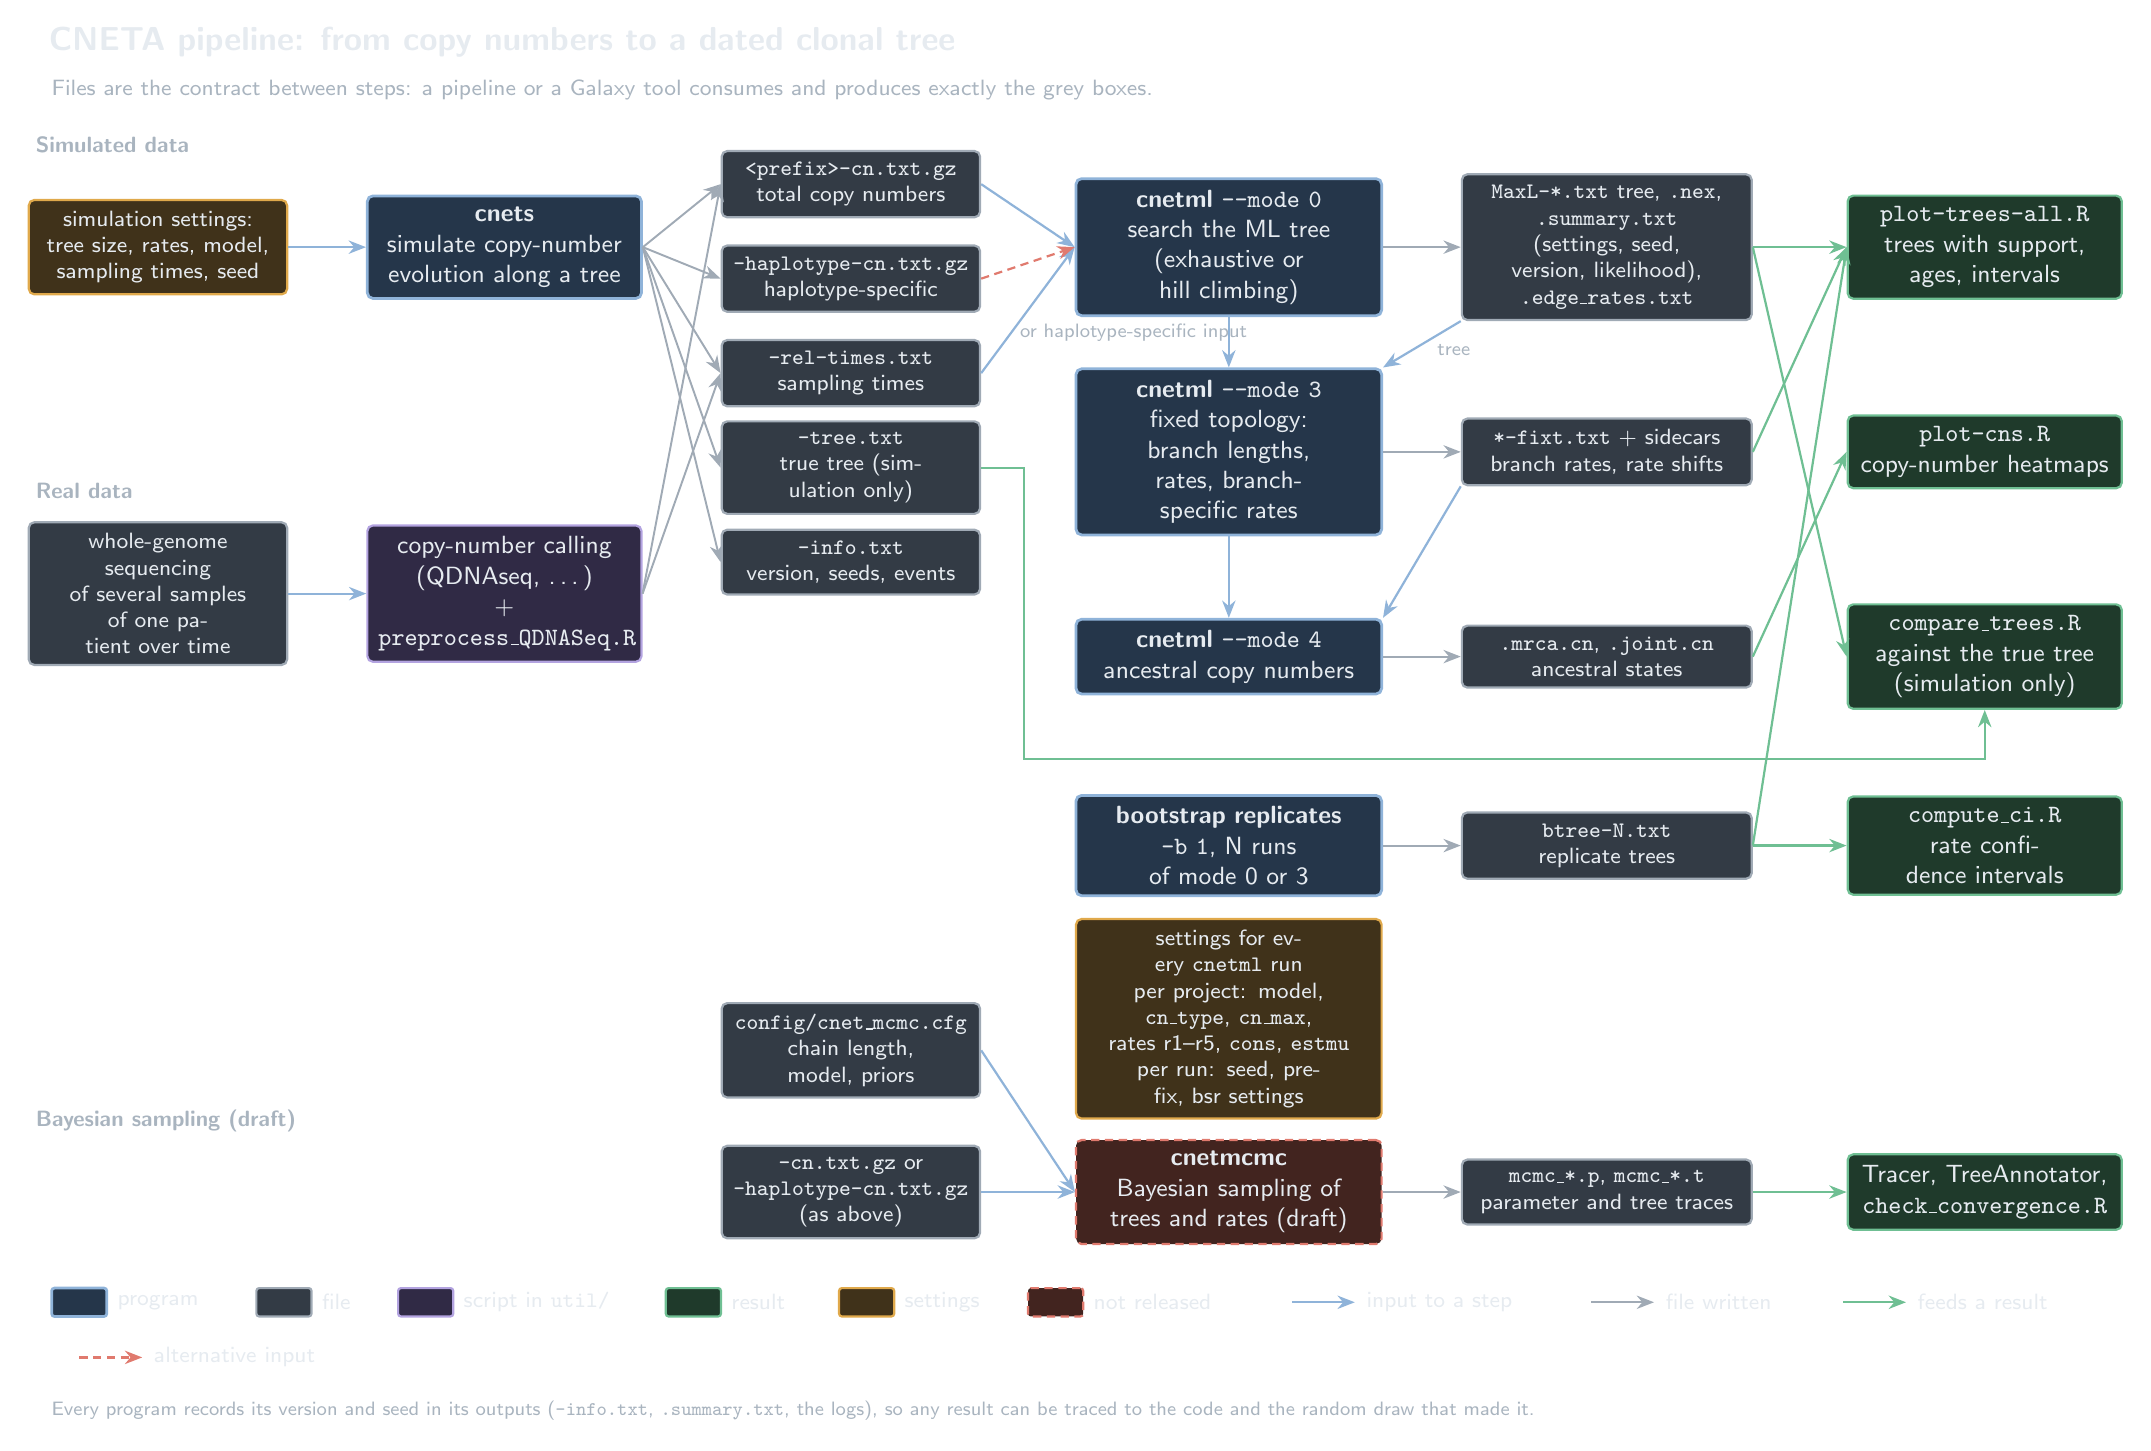
\begin{tikzpicture}

% ---------------------------------------------------------------- title
\node[anchor=west, font=\large\bfseries, inner sep=0pt] at (0,26)
  {CNETA pipeline: from copy numbers to a dated clonal tree};
\node[anchor=west, dcap, font=\footnotesize] at (0,20)
  {Files are the contract between steps: a pipeline or a Galaxy tool consumes and produces exactly the grey boxes.};

% ---------------------------------------------------------------- lanes
\node[lane] at (-2,13) {Simulated data};
\node[lane] at (-2,-31) {Real data};
\node[lane] at (-2,-111) {Bayesian sampling (draft)};

% ---------------------------------------------------------------- column A: sources
\node[settings, text width=30mm] (simset) at (14,0)
  {simulation settings:\\tree size, rates, model,\\sampling times, seed};
\node[file, text width=30mm] (wgs) at (14,-44)
  {whole-genome sequencing\\of several samples\\of one patient over time};

% ---------------------------------------------------------------- column B: producers
\node[prog, text width=32mm] (cnets) at (58,0)
  {\textbf{cnets}\\simulate copy-number\\evolution along a tree};
\node[script, text width=32mm] (prep) at (58,-44)
  {copy-number calling\\(QDNAseq, \ldots)\\+ \f{preprocess\_QDNASeq.R}};

% ---------------------------------------------------------------- column C: input files
\node[file, text width=30mm] (fcn) at (102,8)
  {\f{<prefix>-cn.txt.gz}\\total copy numbers};
\node[file, text width=30mm] (fhap) at (102,-4)
  {\f{-haplotype-cn.txt.gz}\\haplotype-specific};
\node[file, text width=30mm] (ftimes) at (102,-16)
  {\f{-rel-times.txt}\\sampling times};
\node[file, text width=30mm] (ftree) at (102,-28)
  {\f{-tree.txt}\\true tree (simulation only)};
\node[file, text width=30mm] (finfo) at (102,-40)
  {\f{-info.txt}\\version, seeds, events};

% ---------------------------------------------------------------- column D: cnetml
\node[prog, text width=36mm] (m0) at (150,0)
  {\textbf{cnetml} \f{--mode 0}\\search the ML tree\\(exhaustive or hill climbing)};
\node[prog, text width=36mm] (m3) at (150,-26)
  {\textbf{cnetml} \f{--mode 3}\\fixed topology: branch lengths,\\rates, branch-specific rates};
\node[prog, text width=36mm] (m4) at (150,-52)
  {\textbf{cnetml} \f{--mode 4}\\ancestral copy numbers};
\node[prog, text width=36mm] (boot) at (150,-76)
  {\textbf{bootstrap replicates}\\\f{-b 1}, N runs of mode 0 or 3};
\node[settings, text width=36mm] (params) at (150,-98)
  {settings for every \f{cnetml} run\\per project: model, \f{cn\_type}, \f{cn\_max},\\rates r1--r5, \f{cons}, \f{estmu}\\per run: seed, prefix, bsr settings};

% ---------------------------------------------------------------- column E: outputs
\node[file, text width=34mm] (o0) at (198,0)
  {\f{MaxL-*.txt} tree, \f{.nex},\\\f{.summary.txt} (settings, seed,\\version, likelihood), \f{.edge\_rates.txt}};
\node[file, text width=34mm] (o3) at (198,-26)
  {\f{*-fixt.txt} + sidecars\\branch rates, rate shifts};
\node[file, text width=34mm] (o4) at (198,-52)
  {\f{.mrca.cn}, \f{.joint.cn}\\ancestral states};
\node[file, text width=34mm] (ob) at (198,-76)
  {\f{btree-N.txt}\\replicate trees};

% ---------------------------------------------------------------- column F: analysis
\node[result, text width=32mm] (plott) at (246,0)
  {\f{plot-trees-all.R}\\trees with support,\\ages, intervals};
\node[result, text width=32mm] (plotc) at (246,-26)
  {\f{plot-cns.R}\\copy-number heatmaps};
\node[result, text width=32mm] (cmp) at (246,-52)
  {\f{compare\_trees.R}\\against the true tree\\(simulation only)};
\node[result, text width=32mm] (ci) at (246,-76)
  {\f{compute\_ci.R}\\rate confidence intervals};

% ---------------------------------------------------------------- MCMC lane
\node[file, text width=30mm] (cfg) at (102,-102)
  {\f{config/cnet\_mcmc.cfg}\\chain length, model, priors};
\node[file, text width=30mm] (cnin) at (102,-120)
  {\f{-cn.txt.gz} or\\\f{-haplotype-cn.txt.gz}\\(as above)};
\node[draft, text width=36mm] (mcmc) at (150,-120)
  {\textbf{cnetmcmc}\\Bayesian sampling of\\trees and rates (draft)};
\node[file, text width=34mm] (traces) at (198,-120)
  {\f{mcmc\_*.p}, \f{mcmc\_*.t}\\parameter and tree traces};
\node[result, text width=32mm] (tracer) at (246,-120)
  {Tracer, TreeAnnotator,\\\f{check\_convergence.R}};

% ---------------------------------------------------------------- arrows
\draw[arr] (simset) -- (cnets);
\foreach \t in {fcn,fhap,ftimes,ftree,finfo} {\draw[arrf] (cnets.east) -- (\t.west);}
\draw[arr] (wgs) -- (prep);
\draw[arrf] (prep.east) -- (fcn.west);
\draw[arrf] (prep.east) -- (ftimes.west);

\draw[arr] (fcn.east) -- (m0.west);
\draw[arr] (ftimes.east) -- (m0.west);
\draw[arrd] (fhap.east) -- (m0.west);
\node[dcap,anchor=south west] at (123,-12.5) {or haplotype-specific input};

\draw[arrf] (m0) -- (o0);
\draw[arr] (o0.south west) -- (m3.north east);
\node[dcap,anchor=west] at (176,-13) {tree};
\draw[arrf] (m3) -- (o3);
\draw[arr] (o3.south west) -- (m4.north east);
\draw[arrf] (m4) -- (o4);
\draw[arrf] (boot) -- (ob);
\draw[arr] (m0) -- (m3);
\draw[arr] (m3) -- (m4);

\draw[arro] (o0.east) -- (plott.west);
\draw[arro] (o3.east) -- (plott.west);
\draw[arro] (ob.east) -- (plott.west);
\draw[arro] (ob.east) -- (ci.west);
\draw[arro] (o4.east) -- (plotc.west);
\draw[arro] (o0.east) -- (cmp.west);
\draw[arro] (ftree.east) -- (124,-28) -- (124,-65) -- (246,-65) -- (cmp.south);

\draw[arr] (cfg.east) -- (mcmc.west);
\draw[arr] (cnin.east) -- (mcmc.west);
\draw[arrf] (mcmc) -- (traces);
\draw[arro] (traces) -- (tracer);

% ---------------------------------------------------------------- legend
\begin{scope}[shift={(0,-134)}]
  \node[prog, chip]     (lg1) at (4,0)   {}; \node[lg] at ([xshift=2pt]lg1.east) {program};
  \node[file, chip]     (lg2) at (30,0)  {}; \node[lg] at ([xshift=2pt]lg2.east) {file};
  \node[script, chip]   (lg3) at (48,0)  {}; \node[lg] at ([xshift=2pt]lg3.east) {script in \f{util/}};
  \node[result, chip]   (lg4) at (82,0)  {}; \node[lg] at ([xshift=2pt]lg4.east) {result};
  \node[settings, chip] (lg5) at (104,0) {}; \node[lg] at ([xshift=2pt]lg5.east) {settings};
  \node[draft, chip]    (lg6) at (128,0) {}; \node[lg] at ([xshift=2pt]lg6.east) {not released};
  \draw[arr]  (158,0) -- ++(8,0); \node[lg] at (167,0) {input to a step};
  \draw[arrf] (196,0) -- ++(8,0); \node[lg] at (205,0) {file written};
  \draw[arro] (228,0) -- ++(8,0); \node[lg] at (237,0) {feeds a result};
  \draw[arrd] (4,-7) -- ++(8,0);  \node[lg] at (13,-7) {alternative input};
\end{scope}

% ---------------------------------------------------------------- footer
\node[dcap,anchor=north west, align=left] at (0,-146)
  {Every program records its version and seed in its outputs (\f{-info.txt}, \f{.summary.txt}, the logs), so any result can be traced to the code and the random draw that made it.};

\end{tikzpicture}
\end{document}
"
%
%   \PipelineScheme  light | dark   (default light): colours for a light or a
%                    dark background; the background itself stays transparent.
%
% Box colours follow the house convention of the report kit:
%   blue   a program step        grey    a file (the contract between steps)
%   purple a script in util/     green   a result people look at
%   amber  settings to choose    red, dashed   not released yet

\providecommand\PipelineScheme{light}

\documentclass[tikz,border=5mm]{standalone}
\usepackage[T1]{fontenc}
\usepackage{lmodern}
\renewcommand*\familydefault{\sfdefault}
\usetikzlibrary{arrows.meta,positioning,calc,shapes.misc}
\hyphenpenalty=10000
\exhyphenpenalty=10000

% ---------------------------------------------------------------- palette
\def\schemeLight{light}
\ifx\PipelineScheme\schemeLight
  \definecolor{ink}{HTML}{16222E}  \definecolor{muted}{HTML}{6B7280}
  \definecolor{stln}{HTML}{24405C} \definecolor{stfl}{HTML}{E7EEF5}  % program
  \definecolor{syln}{HTML}{55606D} \definecolor{syfl}{HTML}{EDEFF2}  % file
  \definecolor{deln}{HTML}{A5690C} \definecolor{defl}{HTML}{FDF3E2}  % settings
  \definecolor{galn}{HTML}{A83226} \definecolor{gafl}{HTML}{FAE9E7}  % draft
  \definecolor{opln}{HTML}{2C6B4F} \definecolor{opfl}{HTML}{E6F1EB}  % result
  \definecolor{ppln}{HTML}{5B4B8A} \definecolor{ppfl}{HTML}{EEEAF6}  % script
\else
  \definecolor{ink}{HTML}{E6EBF0}  \definecolor{muted}{HTML}{A9B4BF}
  \definecolor{stln}{HTML}{8FB3D9} \definecolor{stfl}{HTML}{25364A}
  \definecolor{syln}{HTML}{A0AAB5} \definecolor{syfl}{HTML}{333B45}
  \definecolor{deln}{HTML}{E0A94B} \definecolor{defl}{HTML}{40321A}
  \definecolor{galn}{HTML}{E07A6E} \definecolor{gafl}{HTML}{42241F}
  \definecolor{opln}{HTML}{6FBF93} \definecolor{opfl}{HTML}{1F3A2B}
  \definecolor{ppln}{HTML}{B3A3E0} \definecolor{ppfl}{HTML}{302A45}
\fi

% ---------------------------------------------------------------- styles
\tikzset{
  x=1mm, y=1mm,
  every node/.style={text=ink, font=\small, align=center, inner sep=4pt,
                     rounded corners=2pt, line width=0.8pt},
  prog/.style={draw=stln, fill=stfl, line width=1pt},
  file/.style={draw=syln, fill=syfl, font=\footnotesize},
  script/.style={draw=ppln, fill=ppfl},
  result/.style={draw=opln, fill=opfl},
  settings/.style={draw=deln, fill=defl, font=\footnotesize},
  draft/.style={draw=galn, fill=gafl, dash pattern=on 3pt off 2pt},
  dcap/.style={text=muted, font=\scriptsize, inner sep=1pt},
  lane/.style={text=muted, font=\footnotesize\bfseries, inner sep=1pt, anchor=west},
  arr/.style={-{Stealth[length=2.2mm,width=1.7mm]}, line width=0.8pt, draw=stln},
  arrf/.style={-{Stealth[length=2.2mm,width=1.7mm]}, line width=0.7pt, draw=syln},
  arro/.style={-{Stealth[length=2.2mm,width=1.7mm]}, line width=0.8pt, draw=opln},
  arrd/.style={-{Stealth[length=2.2mm,width=1.7mm]}, line width=0.8pt, draw=galn,
               dash pattern=on 3pt off 2pt},
  tt/.style={font=\footnotesize\ttfamily},
  % legend swatch: a small box in one of the styles above
  chip/.style={minimum width=7mm, minimum height=3.6mm, inner sep=0pt,
               rounded corners=1pt},
  lg/.style={anchor=west, text=ink, font=\footnotesize, inner sep=1pt},
}
\newcommand{\f}[1]{{\ttfamily #1}}

\begin{document}
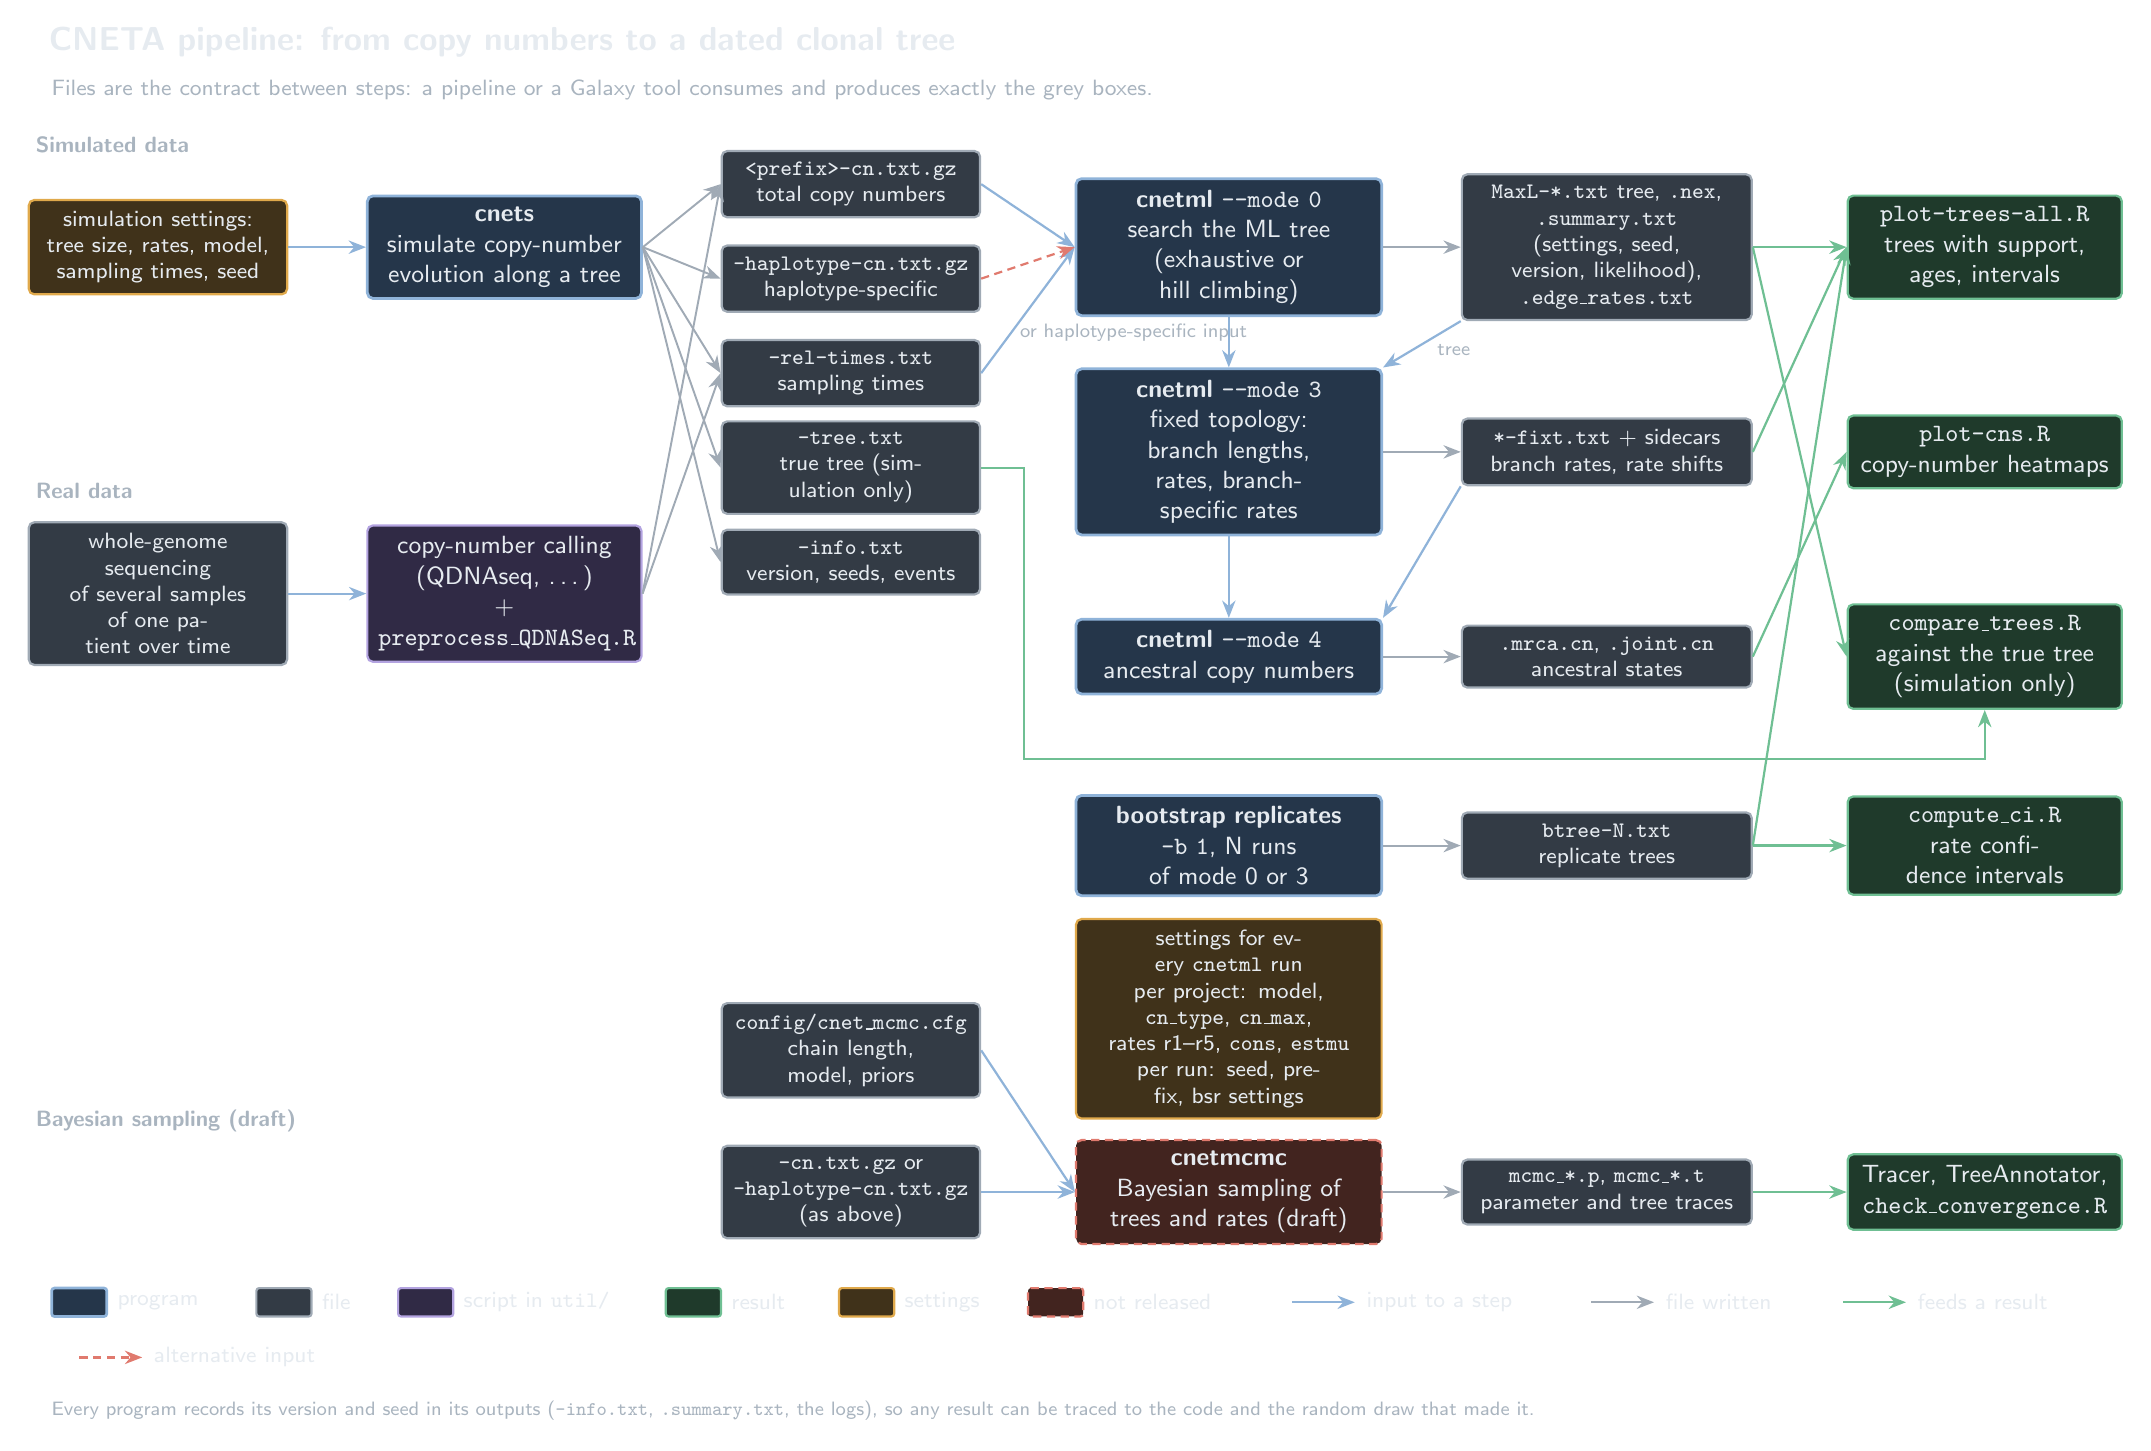
\begin{tikzpicture}

% ---------------------------------------------------------------- title
\node[anchor=west, font=\large\bfseries, inner sep=0pt] at (0,26)
  {CNETA pipeline: from copy numbers to a dated clonal tree};
\node[anchor=west, dcap, font=\footnotesize] at (0,20)
  {Files are the contract between steps: a pipeline or a Galaxy tool consumes and produces exactly the grey boxes.};

% ---------------------------------------------------------------- lanes
\node[lane] at (-2,13) {Simulated data};
\node[lane] at (-2,-31) {Real data};
\node[lane] at (-2,-111) {Bayesian sampling (draft)};

% ---------------------------------------------------------------- column A: sources
\node[settings, text width=30mm] (simset) at (14,0)
  {simulation settings:\\tree size, rates, model,\\sampling times, seed};
\node[file, text width=30mm] (wgs) at (14,-44)
  {whole-genome sequencing\\of several samples\\of one patient over time};

% ---------------------------------------------------------------- column B: producers
\node[prog, text width=32mm] (cnets) at (58,0)
  {\textbf{cnets}\\simulate copy-number\\evolution along a tree};
\node[script, text width=32mm] (prep) at (58,-44)
  {copy-number calling\\(QDNAseq, \ldots)\\+ \f{preprocess\_QDNASeq.R}};

% ---------------------------------------------------------------- column C: input files
\node[file, text width=30mm] (fcn) at (102,8)
  {\f{<prefix>-cn.txt.gz}\\total copy numbers};
\node[file, text width=30mm] (fhap) at (102,-4)
  {\f{-haplotype-cn.txt.gz}\\haplotype-specific};
\node[file, text width=30mm] (ftimes) at (102,-16)
  {\f{-rel-times.txt}\\sampling times};
\node[file, text width=30mm] (ftree) at (102,-28)
  {\f{-tree.txt}\\true tree (simulation only)};
\node[file, text width=30mm] (finfo) at (102,-40)
  {\f{-info.txt}\\version, seeds, events};

% ---------------------------------------------------------------- column D: cnetml
\node[prog, text width=36mm] (m0) at (150,0)
  {\textbf{cnetml} \f{--mode 0}\\search the ML tree\\(exhaustive or hill climbing)};
\node[prog, text width=36mm] (m3) at (150,-26)
  {\textbf{cnetml} \f{--mode 3}\\fixed topology: branch lengths,\\rates, branch-specific rates};
\node[prog, text width=36mm] (m4) at (150,-52)
  {\textbf{cnetml} \f{--mode 4}\\ancestral copy numbers};
\node[prog, text width=36mm] (boot) at (150,-76)
  {\textbf{bootstrap replicates}\\\f{-b 1}, N runs of mode 0 or 3};
\node[settings, text width=36mm] (params) at (150,-98)
  {settings for every \f{cnetml} run\\per project: model, \f{cn\_type}, \f{cn\_max},\\rates r1--r5, \f{cons}, \f{estmu}\\per run: seed, prefix, bsr settings};

% ---------------------------------------------------------------- column E: outputs
\node[file, text width=34mm] (o0) at (198,0)
  {\f{MaxL-*.txt} tree, \f{.nex},\\\f{.summary.txt} (settings, seed,\\version, likelihood), \f{.edge\_rates.txt}};
\node[file, text width=34mm] (o3) at (198,-26)
  {\f{*-fixt.txt} + sidecars\\branch rates, rate shifts};
\node[file, text width=34mm] (o4) at (198,-52)
  {\f{.mrca.cn}, \f{.joint.cn}\\ancestral states};
\node[file, text width=34mm] (ob) at (198,-76)
  {\f{btree-N.txt}\\replicate trees};

% ---------------------------------------------------------------- column F: analysis
\node[result, text width=32mm] (plott) at (246,0)
  {\f{plot-trees-all.R}\\trees with support,\\ages, intervals};
\node[result, text width=32mm] (plotc) at (246,-26)
  {\f{plot-cns.R}\\copy-number heatmaps};
\node[result, text width=32mm] (cmp) at (246,-52)
  {\f{compare\_trees.R}\\against the true tree\\(simulation only)};
\node[result, text width=32mm] (ci) at (246,-76)
  {\f{compute\_ci.R}\\rate confidence intervals};

% ---------------------------------------------------------------- MCMC lane
\node[file, text width=30mm] (cfg) at (102,-102)
  {\f{config/cnet\_mcmc.cfg}\\chain length, model, priors};
\node[file, text width=30mm] (cnin) at (102,-120)
  {\f{-cn.txt.gz} or\\\f{-haplotype-cn.txt.gz}\\(as above)};
\node[draft, text width=36mm] (mcmc) at (150,-120)
  {\textbf{cnetmcmc}\\Bayesian sampling of\\trees and rates (draft)};
\node[file, text width=34mm] (traces) at (198,-120)
  {\f{mcmc\_*.p}, \f{mcmc\_*.t}\\parameter and tree traces};
\node[result, text width=32mm] (tracer) at (246,-120)
  {Tracer, TreeAnnotator,\\\f{check\_convergence.R}};

% ---------------------------------------------------------------- arrows
\draw[arr] (simset) -- (cnets);
\foreach \t in {fcn,fhap,ftimes,ftree,finfo} {\draw[arrf] (cnets.east) -- (\t.west);}
\draw[arr] (wgs) -- (prep);
\draw[arrf] (prep.east) -- (fcn.west);
\draw[arrf] (prep.east) -- (ftimes.west);

\draw[arr] (fcn.east) -- (m0.west);
\draw[arr] (ftimes.east) -- (m0.west);
\draw[arrd] (fhap.east) -- (m0.west);
\node[dcap,anchor=south west] at (123,-12.5) {or haplotype-specific input};

\draw[arrf] (m0) -- (o0);
\draw[arr] (o0.south west) -- (m3.north east);
\node[dcap,anchor=west] at (176,-13) {tree};
\draw[arrf] (m3) -- (o3);
\draw[arr] (o3.south west) -- (m4.north east);
\draw[arrf] (m4) -- (o4);
\draw[arrf] (boot) -- (ob);
\draw[arr] (m0) -- (m3);
\draw[arr] (m3) -- (m4);

\draw[arro] (o0.east) -- (plott.west);
\draw[arro] (o3.east) -- (plott.west);
\draw[arro] (ob.east) -- (plott.west);
\draw[arro] (ob.east) -- (ci.west);
\draw[arro] (o4.east) -- (plotc.west);
\draw[arro] (o0.east) -- (cmp.west);
\draw[arro] (ftree.east) -- (124,-28) -- (124,-65) -- (246,-65) -- (cmp.south);

\draw[arr] (cfg.east) -- (mcmc.west);
\draw[arr] (cnin.east) -- (mcmc.west);
\draw[arrf] (mcmc) -- (traces);
\draw[arro] (traces) -- (tracer);

% ---------------------------------------------------------------- legend
\begin{scope}[shift={(0,-134)}]
  \node[prog, chip]     (lg1) at (4,0)   {}; \node[lg] at ([xshift=2pt]lg1.east) {program};
  \node[file, chip]     (lg2) at (30,0)  {}; \node[lg] at ([xshift=2pt]lg2.east) {file};
  \node[script, chip]   (lg3) at (48,0)  {}; \node[lg] at ([xshift=2pt]lg3.east) {script in \f{util/}};
  \node[result, chip]   (lg4) at (82,0)  {}; \node[lg] at ([xshift=2pt]lg4.east) {result};
  \node[settings, chip] (lg5) at (104,0) {}; \node[lg] at ([xshift=2pt]lg5.east) {settings};
  \node[draft, chip]    (lg6) at (128,0) {}; \node[lg] at ([xshift=2pt]lg6.east) {not released};
  \draw[arr]  (158,0) -- ++(8,0); \node[lg] at (167,0) {input to a step};
  \draw[arrf] (196,0) -- ++(8,0); \node[lg] at (205,0) {file written};
  \draw[arro] (228,0) -- ++(8,0); \node[lg] at (237,0) {feeds a result};
  \draw[arrd] (4,-7) -- ++(8,0);  \node[lg] at (13,-7) {alternative input};
\end{scope}

% ---------------------------------------------------------------- footer
\node[dcap,anchor=north west, align=left] at (0,-146)
  {Every program records its version and seed in its outputs (\f{-info.txt}, \f{.summary.txt}, the logs), so any result can be traced to the code and the random draw that made it.};

\end{tikzpicture}
\end{document}
"
%
%   \PipelineScheme  light | dark   (default light): colours for a light or a
%                    dark background; the background itself stays transparent.
%
% Box colours follow the house convention of the report kit:
%   blue   a program step        grey    a file (the contract between steps)
%   purple a script in util/     green   a result people look at
%   amber  settings to choose    red, dashed   not released yet

\providecommand\PipelineScheme{light}

\documentclass[tikz,border=5mm]{standalone}
\usepackage[T1]{fontenc}
\usepackage{lmodern}
\renewcommand*\familydefault{\sfdefault}
\usetikzlibrary{arrows.meta,positioning,calc,shapes.misc}
\hyphenpenalty=10000
\exhyphenpenalty=10000

% ---------------------------------------------------------------- palette
\def\schemeLight{light}
\ifx\PipelineScheme\schemeLight
  \definecolor{ink}{HTML}{16222E}  \definecolor{muted}{HTML}{6B7280}
  \definecolor{stln}{HTML}{24405C} \definecolor{stfl}{HTML}{E7EEF5}  % program
  \definecolor{syln}{HTML}{55606D} \definecolor{syfl}{HTML}{EDEFF2}  % file
  \definecolor{deln}{HTML}{A5690C} \definecolor{defl}{HTML}{FDF3E2}  % settings
  \definecolor{galn}{HTML}{A83226} \definecolor{gafl}{HTML}{FAE9E7}  % draft
  \definecolor{opln}{HTML}{2C6B4F} \definecolor{opfl}{HTML}{E6F1EB}  % result
  \definecolor{ppln}{HTML}{5B4B8A} \definecolor{ppfl}{HTML}{EEEAF6}  % script
\else
  \definecolor{ink}{HTML}{E6EBF0}  \definecolor{muted}{HTML}{A9B4BF}
  \definecolor{stln}{HTML}{8FB3D9} \definecolor{stfl}{HTML}{25364A}
  \definecolor{syln}{HTML}{A0AAB5} \definecolor{syfl}{HTML}{333B45}
  \definecolor{deln}{HTML}{E0A94B} \definecolor{defl}{HTML}{40321A}
  \definecolor{galn}{HTML}{E07A6E} \definecolor{gafl}{HTML}{42241F}
  \definecolor{opln}{HTML}{6FBF93} \definecolor{opfl}{HTML}{1F3A2B}
  \definecolor{ppln}{HTML}{B3A3E0} \definecolor{ppfl}{HTML}{302A45}
\fi

% ---------------------------------------------------------------- styles
\tikzset{
  x=1mm, y=1mm,
  every node/.style={text=ink, font=\small, align=center, inner sep=4pt,
                     rounded corners=2pt, line width=0.8pt},
  prog/.style={draw=stln, fill=stfl, line width=1pt},
  file/.style={draw=syln, fill=syfl, font=\footnotesize},
  script/.style={draw=ppln, fill=ppfl},
  result/.style={draw=opln, fill=opfl},
  settings/.style={draw=deln, fill=defl, font=\footnotesize},
  draft/.style={draw=galn, fill=gafl, dash pattern=on 3pt off 2pt},
  dcap/.style={text=muted, font=\scriptsize, inner sep=1pt},
  lane/.style={text=muted, font=\footnotesize\bfseries, inner sep=1pt, anchor=west},
  arr/.style={-{Stealth[length=2.2mm,width=1.7mm]}, line width=0.8pt, draw=stln},
  arrf/.style={-{Stealth[length=2.2mm,width=1.7mm]}, line width=0.7pt, draw=syln},
  arro/.style={-{Stealth[length=2.2mm,width=1.7mm]}, line width=0.8pt, draw=opln},
  arrd/.style={-{Stealth[length=2.2mm,width=1.7mm]}, line width=0.8pt, draw=galn,
               dash pattern=on 3pt off 2pt},
  tt/.style={font=\footnotesize\ttfamily},
  % legend swatch: a small box in one of the styles above
  chip/.style={minimum width=7mm, minimum height=3.6mm, inner sep=0pt,
               rounded corners=1pt},
  lg/.style={anchor=west, text=ink, font=\footnotesize, inner sep=1pt},
}
\newcommand{\f}[1]{{\ttfamily #1}}

\begin{document}
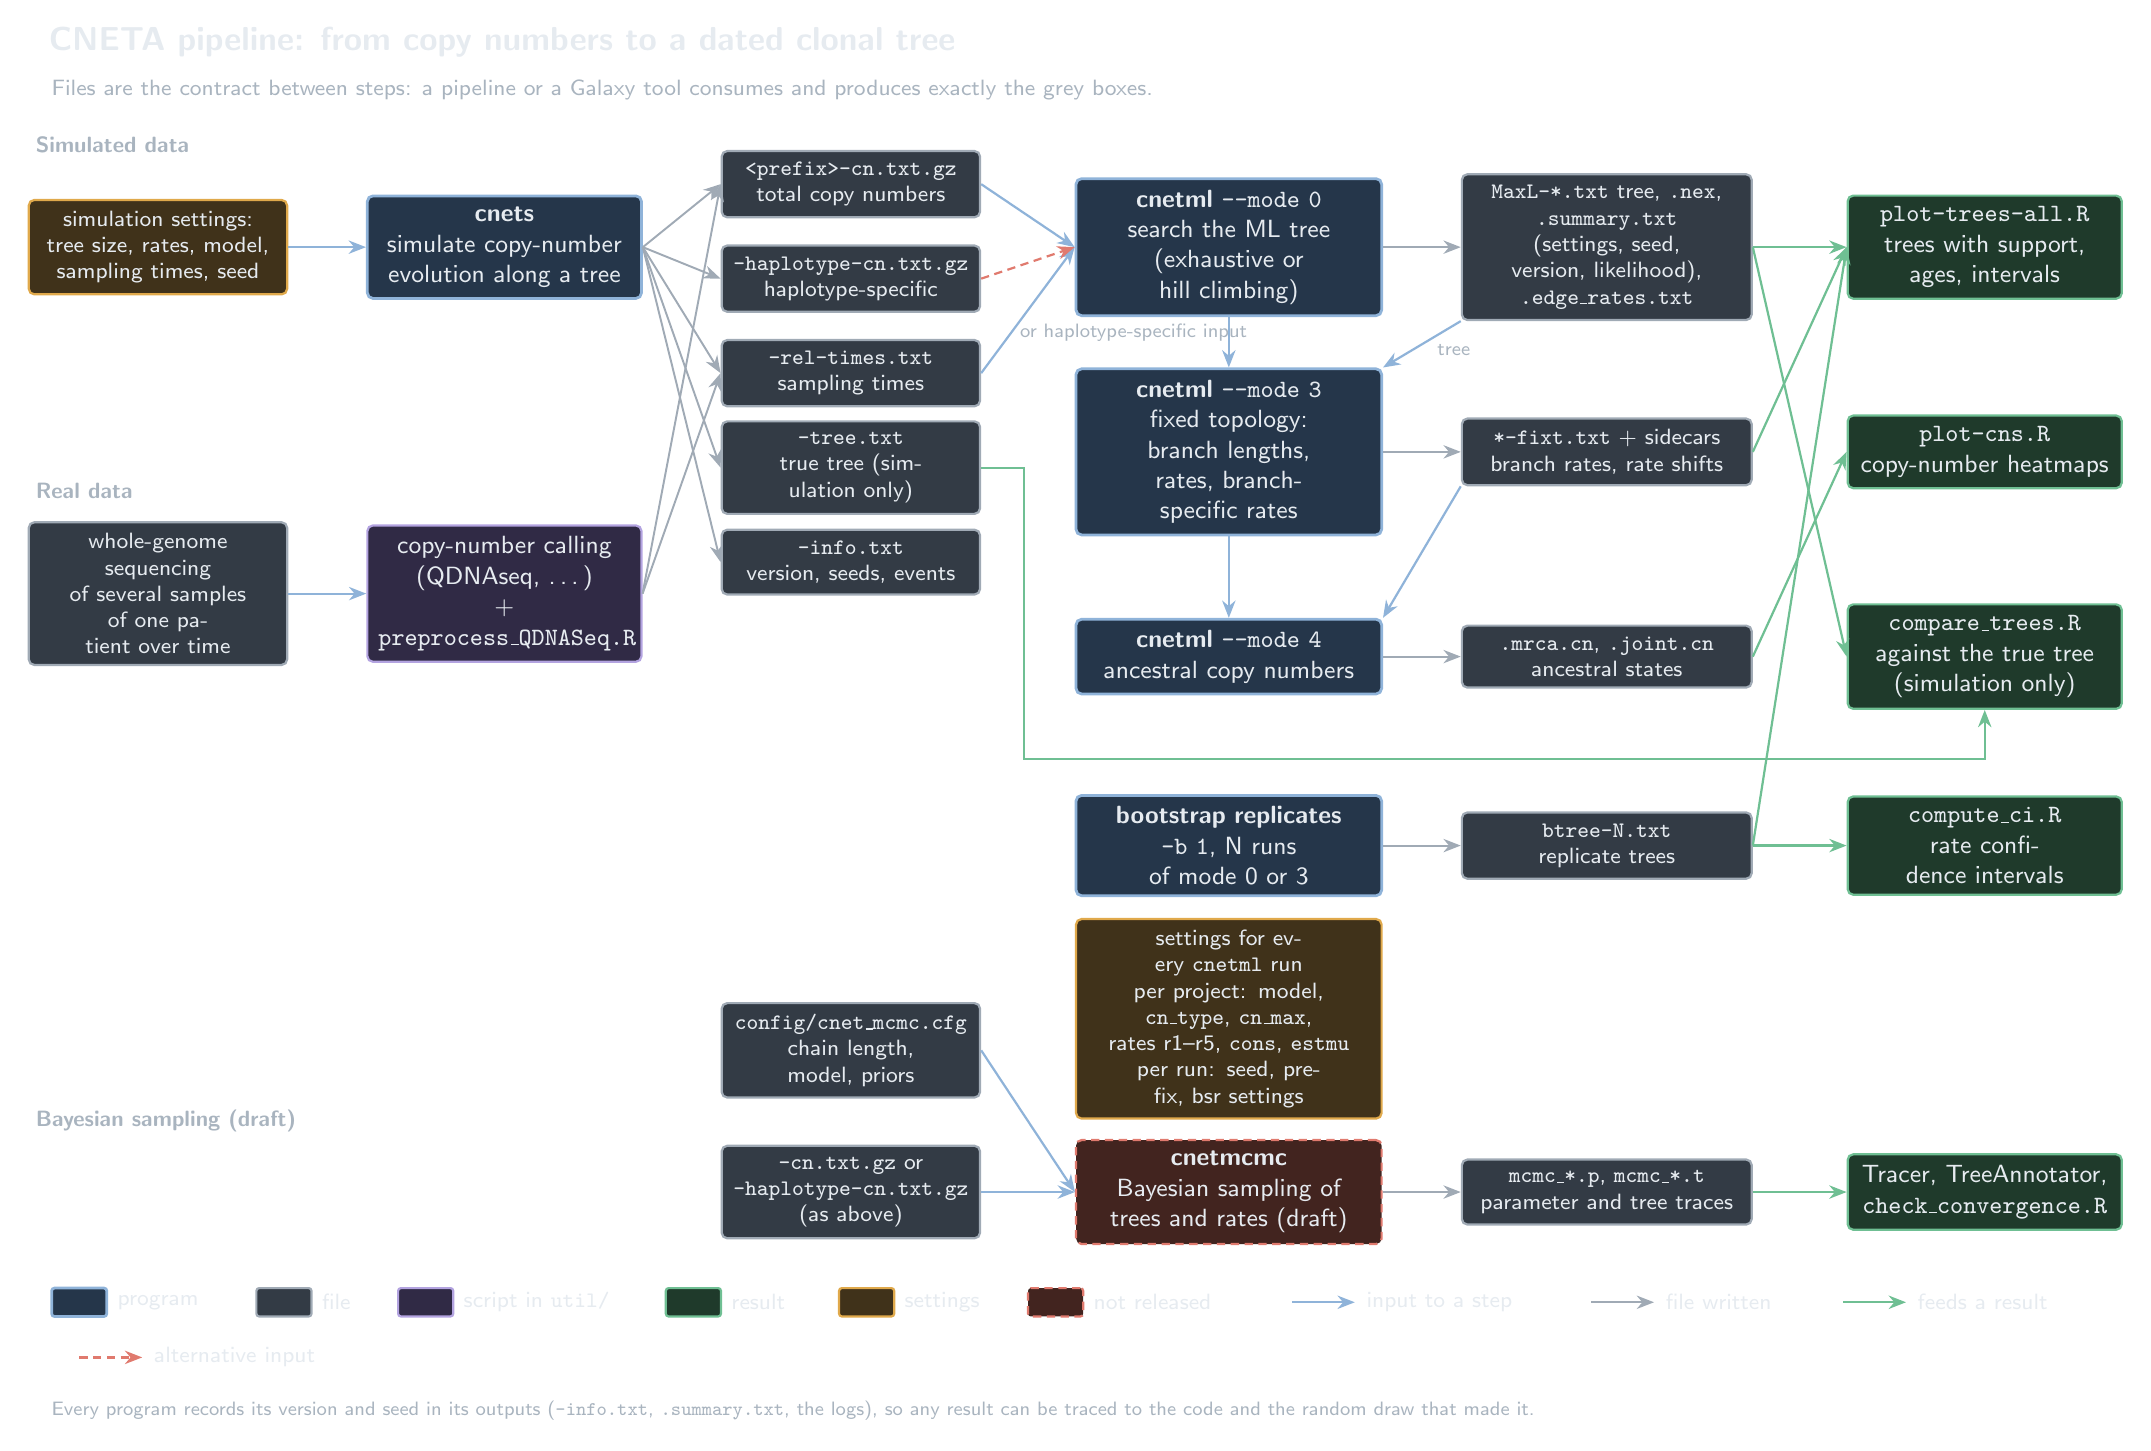
\begin{tikzpicture}

% ---------------------------------------------------------------- title
\node[anchor=west, font=\large\bfseries, inner sep=0pt] at (0,26)
  {CNETA pipeline: from copy numbers to a dated clonal tree};
\node[anchor=west, dcap, font=\footnotesize] at (0,20)
  {Files are the contract between steps: a pipeline or a Galaxy tool consumes and produces exactly the grey boxes.};

% ---------------------------------------------------------------- lanes
\node[lane] at (-2,13) {Simulated data};
\node[lane] at (-2,-31) {Real data};
\node[lane] at (-2,-111) {Bayesian sampling (draft)};

% ---------------------------------------------------------------- column A: sources
\node[settings, text width=30mm] (simset) at (14,0)
  {simulation settings:\\tree size, rates, model,\\sampling times, seed};
\node[file, text width=30mm] (wgs) at (14,-44)
  {whole-genome sequencing\\of several samples\\of one patient over time};

% ---------------------------------------------------------------- column B: producers
\node[prog, text width=32mm] (cnets) at (58,0)
  {\textbf{cnets}\\simulate copy-number\\evolution along a tree};
\node[script, text width=32mm] (prep) at (58,-44)
  {copy-number calling\\(QDNAseq, \ldots)\\+ \f{preprocess\_QDNASeq.R}};

% ---------------------------------------------------------------- column C: input files
\node[file, text width=30mm] (fcn) at (102,8)
  {\f{<prefix>-cn.txt.gz}\\total copy numbers};
\node[file, text width=30mm] (fhap) at (102,-4)
  {\f{-haplotype-cn.txt.gz}\\haplotype-specific};
\node[file, text width=30mm] (ftimes) at (102,-16)
  {\f{-rel-times.txt}\\sampling times};
\node[file, text width=30mm] (ftree) at (102,-28)
  {\f{-tree.txt}\\true tree (simulation only)};
\node[file, text width=30mm] (finfo) at (102,-40)
  {\f{-info.txt}\\version, seeds, events};

% ---------------------------------------------------------------- column D: cnetml
\node[prog, text width=36mm] (m0) at (150,0)
  {\textbf{cnetml} \f{--mode 0}\\search the ML tree\\(exhaustive or hill climbing)};
\node[prog, text width=36mm] (m3) at (150,-26)
  {\textbf{cnetml} \f{--mode 3}\\fixed topology: branch lengths,\\rates, branch-specific rates};
\node[prog, text width=36mm] (m4) at (150,-52)
  {\textbf{cnetml} \f{--mode 4}\\ancestral copy numbers};
\node[prog, text width=36mm] (boot) at (150,-76)
  {\textbf{bootstrap replicates}\\\f{-b 1}, N runs of mode 0 or 3};
\node[settings, text width=36mm] (params) at (150,-98)
  {settings for every \f{cnetml} run\\per project: model, \f{cn\_type}, \f{cn\_max},\\rates r1--r5, \f{cons}, \f{estmu}\\per run: seed, prefix, bsr settings};

% ---------------------------------------------------------------- column E: outputs
\node[file, text width=34mm] (o0) at (198,0)
  {\f{MaxL-*.txt} tree, \f{.nex},\\\f{.summary.txt} (settings, seed,\\version, likelihood), \f{.edge\_rates.txt}};
\node[file, text width=34mm] (o3) at (198,-26)
  {\f{*-fixt.txt} + sidecars\\branch rates, rate shifts};
\node[file, text width=34mm] (o4) at (198,-52)
  {\f{.mrca.cn}, \f{.joint.cn}\\ancestral states};
\node[file, text width=34mm] (ob) at (198,-76)
  {\f{btree-N.txt}\\replicate trees};

% ---------------------------------------------------------------- column F: analysis
\node[result, text width=32mm] (plott) at (246,0)
  {\f{plot-trees-all.R}\\trees with support,\\ages, intervals};
\node[result, text width=32mm] (plotc) at (246,-26)
  {\f{plot-cns.R}\\copy-number heatmaps};
\node[result, text width=32mm] (cmp) at (246,-52)
  {\f{compare\_trees.R}\\against the true tree\\(simulation only)};
\node[result, text width=32mm] (ci) at (246,-76)
  {\f{compute\_ci.R}\\rate confidence intervals};

% ---------------------------------------------------------------- MCMC lane
\node[file, text width=30mm] (cfg) at (102,-102)
  {\f{config/cnet\_mcmc.cfg}\\chain length, model, priors};
\node[file, text width=30mm] (cnin) at (102,-120)
  {\f{-cn.txt.gz} or\\\f{-haplotype-cn.txt.gz}\\(as above)};
\node[draft, text width=36mm] (mcmc) at (150,-120)
  {\textbf{cnetmcmc}\\Bayesian sampling of\\trees and rates (draft)};
\node[file, text width=34mm] (traces) at (198,-120)
  {\f{mcmc\_*.p}, \f{mcmc\_*.t}\\parameter and tree traces};
\node[result, text width=32mm] (tracer) at (246,-120)
  {Tracer, TreeAnnotator,\\\f{check\_convergence.R}};

% ---------------------------------------------------------------- arrows
\draw[arr] (simset) -- (cnets);
\foreach \t in {fcn,fhap,ftimes,ftree,finfo} {\draw[arrf] (cnets.east) -- (\t.west);}
\draw[arr] (wgs) -- (prep);
\draw[arrf] (prep.east) -- (fcn.west);
\draw[arrf] (prep.east) -- (ftimes.west);

\draw[arr] (fcn.east) -- (m0.west);
\draw[arr] (ftimes.east) -- (m0.west);
\draw[arrd] (fhap.east) -- (m0.west);
\node[dcap,anchor=south west] at (123,-12.5) {or haplotype-specific input};

\draw[arrf] (m0) -- (o0);
\draw[arr] (o0.south west) -- (m3.north east);
\node[dcap,anchor=west] at (176,-13) {tree};
\draw[arrf] (m3) -- (o3);
\draw[arr] (o3.south west) -- (m4.north east);
\draw[arrf] (m4) -- (o4);
\draw[arrf] (boot) -- (ob);
\draw[arr] (m0) -- (m3);
\draw[arr] (m3) -- (m4);

\draw[arro] (o0.east) -- (plott.west);
\draw[arro] (o3.east) -- (plott.west);
\draw[arro] (ob.east) -- (plott.west);
\draw[arro] (ob.east) -- (ci.west);
\draw[arro] (o4.east) -- (plotc.west);
\draw[arro] (o0.east) -- (cmp.west);
\draw[arro] (ftree.east) -- (124,-28) -- (124,-65) -- (246,-65) -- (cmp.south);

\draw[arr] (cfg.east) -- (mcmc.west);
\draw[arr] (cnin.east) -- (mcmc.west);
\draw[arrf] (mcmc) -- (traces);
\draw[arro] (traces) -- (tracer);

% ---------------------------------------------------------------- legend
\begin{scope}[shift={(0,-134)}]
  \node[prog, chip]     (lg1) at (4,0)   {}; \node[lg] at ([xshift=2pt]lg1.east) {program};
  \node[file, chip]     (lg2) at (30,0)  {}; \node[lg] at ([xshift=2pt]lg2.east) {file};
  \node[script, chip]   (lg3) at (48,0)  {}; \node[lg] at ([xshift=2pt]lg3.east) {script in \f{util/}};
  \node[result, chip]   (lg4) at (82,0)  {}; \node[lg] at ([xshift=2pt]lg4.east) {result};
  \node[settings, chip] (lg5) at (104,0) {}; \node[lg] at ([xshift=2pt]lg5.east) {settings};
  \node[draft, chip]    (lg6) at (128,0) {}; \node[lg] at ([xshift=2pt]lg6.east) {not released};
  \draw[arr]  (158,0) -- ++(8,0); \node[lg] at (167,0) {input to a step};
  \draw[arrf] (196,0) -- ++(8,0); \node[lg] at (205,0) {file written};
  \draw[arro] (228,0) -- ++(8,0); \node[lg] at (237,0) {feeds a result};
  \draw[arrd] (4,-7) -- ++(8,0);  \node[lg] at (13,-7) {alternative input};
\end{scope}

% ---------------------------------------------------------------- footer
\node[dcap,anchor=north west, align=left] at (0,-146)
  {Every program records its version and seed in its outputs (\f{-info.txt}, \f{.summary.txt}, the logs), so any result can be traced to the code and the random draw that made it.};

\end{tikzpicture}
\end{document}
